\documentclass[10pt,a4paper]{article}
\usepackage[UTF8,fontset = windows]{ctex}
\setCJKmainfont[BoldFont=黑体,ItalicFont=楷体]{华文中宋}
\usepackage{amssymb,amsmath,amsfonts,amsthm,mathrsfs,dsfont,graphicx}
\usepackage{ifthen,indentfirst,enumerate,color,titletoc}
\usepackage{tikz}
\usepackage{makecell}
\usepackage{longtable}
%\usepackage{mathptmx}

\usetikzlibrary{arrows,calc,intersections,patterns,decorations.pathreplacing}
\usepackage[bf,small,indentafter,pagestyles]{titlesec}
\usepackage[top=1in, bottom=1in,left=0.8in,right=0.8in]{geometry}
\renewcommand{\baselinestretch}{1.65}
\newtheorem{defi}{定义~}
\newtheorem{eg}{例~}
\newtheorem{ex}{~}
\newtheorem{rem}{注~}
\newtheorem{thm}{定理~}
\newtheorem{coro}{推论~}
\newtheorem{axiom}{公理~}
\newtheorem{prop}{性质~}
\newcommand{\blank}[1]{\underline{\hbox to #1pt{}}}
\newcommand{\bracket}[1]{(\hbox to #1pt{})}
\newcommand{\onech}[4]{\par\begin{tabular}{p{.9\textwidth}}
A.~#1\\
B.~#2\\
C.~#3\\
D.~#4
\end{tabular}}
\newcommand{\twoch}[4]{\par\begin{tabular}{p{.46\textwidth}p{.46\textwidth}}
A.~#1& B.~#2\\
C.~#3& D.~#4
\end{tabular}}
\newcommand{\vartwoch}[4]{\par\begin{tabular}{p{.46\textwidth}p{.46\textwidth}}
(1)~#1& (2)~#2\\
(3)~#3& (4)~#4
\end{tabular}}
\newcommand{\fourch}[4]{\par\begin{tabular}{p{.23\textwidth}p{.23\textwidth}p{.23\textwidth}p{.23\textwidth}}
A.~#1 &B.~#2& C.~#3& D.~#4
\end{tabular}}
\newcommand{\varfourch}[4]{\par\begin{tabular}{p{.23\textwidth}p{.23\textwidth}p{.23\textwidth}p{.23\textwidth}}
(1)~#1 &(2)~#2& (3)~#3& (4)~#4
\end{tabular}}
\begin{document}
\begin{enumerate}[1.]


\item 已知$\cos \alpha =\dfrac{24}{25}$, 求$\sin \alpha$.		
解答在这里  利用``勾股数'', 若$\alpha$在第一象限, 则$\sin \alpha =\dfrac 7{25}$; 若$\alpha$在第四象限, 则$\sin \alpha =-\dfrac 7{25}$.
\item 已知$\tan \alpha =-\sqrt 5$, 求$\cos \alpha$.
解答在这里 如图, 若$\alpha$在第二象限, 则$\cos \alpha =\dfrac{-1}{\sqrt 6}=-\dfrac{\sqrt 6}6$; 若$\alpha$在第四象限, 则$\cos \alpha =\dfrac 1{\sqrt 6}=\dfrac{\sqrt 6}6$.
\begin{center}
    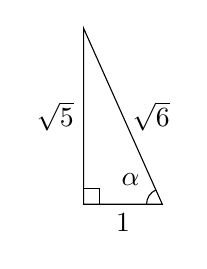
\begin{tikzpicture}
        \draw (0,0) -- (1,0) -- (0,{sqrt(5)}) -- cycle;
        \draw (0.5,0) node [below] {$1$} (0,{sqrt(5)/2}) node [left] {$\sqrt{5}$} (0.5,{sqrt(5)/2}) node [right] {$\sqrt{6}$};
        \draw (0.2,0) -- (0.2,0.2) -- (0,0.2);
        \draw (0.8,0) arc (180:{180-atan(sqrt(5))}:0.2);
        \draw (1,0) ++ ({180-0.5*atan(sqrt(5))}:0.2) node [above left] {$\alpha$};
    \end{tikzpicture}
\end{center}
\item 已知$\cos \alpha =m$($m\ne 0$, $m\ne \pm 1$), 求$\alpha$的其他三角函数值.\\
解答在这里  因为$\sin ^2\alpha +\cos ^2\alpha =1$, 故可按$\sin \alpha$的符号划分象限.
(1) 若$\alpha$在第一、二象限, 则$\sec \alpha =\dfrac 1m$(倒), $\sin \alpha =\sqrt {1-m^2}$(平), $\csc \alpha =\dfrac 1{\sqrt {1-m^2}}$(倒), $\tan \alpha =\dfrac{\sin \alpha}{\cos \alpha}=\dfrac{\sqrt {1-m^2}}m$(商), $\cot \alpha =\dfrac m{\sqrt {1-m^2}}$(倒).
(2) 若$\alpha$在第二、四象限, 则$\sec \alpha =\dfrac 1m$, $\sin \alpha =-\sqrt {1-m^2}$, $\csc \alpha =-\dfrac 1{\sqrt {1-m^2}}$, $\tan \alpha =-\dfrac{\sqrt {1-m^2}}m$, $\cot \alpha =-\dfrac m{\sqrt {1-m^2}}$.
\item 求证: $\dfrac{1-\tan ^2x}{1+\tan ^2x}=\cos ^2x-\sin ^2x$.\\
解答在这里  因为$ \dfrac{1-\tan ^2x}{1+\tan ^2x}=\dfrac{1-\dfrac{\sin ^2x}{\cos ^2x}}{1+\dfrac{\sin ^2x}{\cos ^2x}}=\dfrac{\cos ^2x-\sin ^2x}{\cos ^2x+\sin ^2x}=\cos ^2x-\sin ^2x$, 左边$=$右边, 所以原式成立.
\item 求证: $\dfrac{\tan \alpha}{\tan \alpha -\tan \beta}=\dfrac{\cot \beta}{\cot \beta -\cot \alpha}$.\\
解答在这里 因为$\dfrac{\cot \beta}{\cot \beta -\cot \alpha}=\dfrac{\cot \beta (\tan \alpha \tan \beta)}{(\cot \beta -\cot \alpha)(\tan \alpha \tan \beta)}=\dfrac{\tan \alpha (\cot \beta \tan \beta)}{\tan \alpha (\cot \beta \tan \beta)-(\cot \alpha \tan \alpha)\tan \beta}$
$=\dfrac{\tan \alpha}{\tan \alpha -\tan \beta}$, 左边$=$右边, 所以原式成立.
\item 求证: $\sin ^21^\circ +\sin ^22^\circ +\cdots +\sin ^289^\circ =\dfrac{89}2$.\\
解答在这里  因为$ \sin ^289^\circ =\cos ^21^\circ$, $\sin ^288^\circ =\cos ^22^\circ$, …, $\sin ^246^\circ =\cos ^244^\circ$,
所以左边$=(\sin ^21^\circ +\cos ^21^\circ)+(\sin ^22^\circ +\cos ^22^\circ)+\cdots +(\sin ^244^\circ +\cos ^244^\circ)+\sin ^245^\circ$
$=44+\dfrac 12=\dfrac{89}2$. 所以原式成立.
\item 求证$\dfrac{1+2\sin \alpha \cos \alpha \cos ^2\alpha -\sin ^2\alpha =\dfrac 1+\tan \alpha}{1-\tan \alpha}$.\\
解答在这里 因为左边$=\dfrac{\sin ^2\alpha +2\sin \alpha \cos \alpha +\cos ^2\alpha \cos ^2\alpha -\sin ^2\alpha =\dfrac (\cos \alpha +\sin \alpha)^2}{(\cos \alpha +\sin \alpha)(\cos \alpha -\sin \alpha)}=\dfrac{\cos \alpha +\sin \alpha}{\cos \alpha -\sin \alpha}=\dfrac{1+\tan \alpha}{1-\tan \alpha}$, 所以原式成立.
\item 求证$\dfrac{1+\sec \alpha +\tan \alpha}{1+\sec \alpha -\tan \alpha}=\dfrac{1+\sin \alpha}{\cos \alpha}$.
解答在这里 因为$ \dfrac{1+\sec \alpha +\tan \alpha}{1+\sec \alpha -\tan \alpha}=\dfrac{(\sec ^2\alpha -\tan ^2\alpha)+(\sec \alpha +\tan \alpha)}{\sec \alpha +1-\tan \alpha}=\dfrac{(\sec \alpha +\tan \alpha)(\sec \alpha -\tan \alpha)+(\sec \alpha +\tan \alpha)}{\sec \alpha +1-\tan \alpha}=\dfrac{(\sec \alpha +\tan \alpha)(\sec \alpha -\tan \alpha +1)}{\sec \alpha +1-\tan \alpha}=\sec \alpha +\tan \alpha =\dfrac 1{\cos \alpha}+\dfrac{\sin \alpha}{\cos \alpha}=\dfrac{1+\sin \alpha}{\cos \alpha}$, 所以原式成立.
\item 已知$\tan \theta =-3$, 求下列各式的值:\\
(1) $3\sin \theta +\cos \theta$;\\
(2)$\sin ^2\theta -2\sin \theta \cos \theta +1$.\\
解答在这里  (1)$3\sin \theta +\cos \theta =\cos \theta (3\tan \theta +1)=\pm \dfrac 1{\sqrt {10}}(-9+1)=\pm \dfrac 8{\sqrt {10}}=\pm \dfrac 45\sqrt {10}$.
(2)$\sin ^2\theta -2\sin \theta \cos \theta +1=\dfrac{2\sin ^2\theta -2\sin \theta \cos \theta +\cos ^2\theta}{\sin ^2\theta +\cos ^2\theta}=\dfrac{2\tan ^2\theta -2\tan \theta +1}{\tan ^2\theta +1}=\dfrac{18+6+1}{9+1}=\dfrac 52$.
\item 在\textcircled{1} $160^\circ$, \textcircled{2} $480^\circ$, \textcircled{3} $-960^\circ$, \textcircled{4} $-1600^\circ$这四个角中, 属于第二象限的角有\bracket{20}.
\fourch{\textcircled{1}}{\textcircled{1}\textcircled{2}}{\textcircled{1}\textcircled{2}\textcircled{3}}{\textcircled{1}\textcircled{2}\textcircled{3}\textcircled{4}}
\item 集合$M=\{\alpha|\alpha =k\cdot 90^\circ , \ k\in \mathbf{N}\}$中各角的终边都在\bracket{20}.
\twoch{$x$轴的正半轴上}{$y$轴的正半轴上}{$x$轴或$y$轴上}{$x$轴正半轴或$y$轴的正半轴上}
\item 若$\alpha$是第四象限的角, 则$\pi -\alpha$是\bracket{20}.
\fourch{第一象限的角}{第二象限的角}{第三象限的角}{第四象限的角}
\item 若一圆弧长等于其所在圆的内接正三角形的边长, 则其圆心角的弧度数为\bracket{20}.
\fourch{$\dfrac{\pi}3$}{$\dfrac 23\pi$}{$\sqrt 3$}{$2$}
\item 若$\alpha$和$\beta$的终边关于$y$轴对称, 则必有\bracket{20}.
\twoch{$\alpha +\beta =\dfrac{\pi}2$}{$\alpha +\beta =(2k+\dfrac 12)\pi$($k\in \mathbf{Z}$)}{$\alpha +\beta =2k\pi$($k\in \mathbf{Z}$)}{$\alpha +\beta =(2k+1)\pi$($k\in \mathbf{Z}$)}
\item 若$-\dfrac{\pi}2<\alpha <\beta <\dfrac{\pi}2$, 则$\alpha -\beta$的取值范围是\bracket{20}.
\fourch{$(-\dfrac{\pi}2,0)$}{$(-\dfrac{\pi}2,\dfrac{\pi}2)$}{$(-\pi ,0)$}{$(-\pi ,\pi)$}
\item 集合$M=\{x|x=\dfrac{k\pi}2\pm \dfrac{\pi}4,\ k\in \mathbf{Z}\}$与$P=\{x|x=\dfrac{k\pi}4,\ k\in \mathbf{Z}\}$之间的关系是\bracket{20}.
\fourch{$M\subset P$}{$M\supset P$}{$M=P$}{$M\cap P=\varnothing$}
\item 与$-45^\circ$角终边相同的角的集合是\blank{50}.
\item 若$\alpha$是第四象限的角, 则$\alpha$的取值范围是\blank{50}.
\item 终边落在$x$轴负半轴上的角的集合为\blank{50}.
\item 终边落在第一、三象限角平分线上的角的集合为\blank{50}.
\item 若角$\alpha$与$\beta$的终边是互为反向延长线, 则$\alpha$, $\beta$之间满足关系式是\blank{50}.
\item 若角$\alpha$的终边和函数$y=-|x|$的图像重合, 则$\alpha$的集合是\blank{50}.
\item 若$\alpha$是第二象限的角, 则$\dfrac{\alpha}2$是第\blank{50}象限的角, $2\alpha$是第\blank{50}象限的角.
\item 若$\alpha =-4$, 则$\alpha$是第\blank{50}象限的角.
\item 在$-720^\circ$与$720^\circ$之间, 与$60^\circ$角终边相同的角是\blank{50}.
\item 设角$\alpha$的终边与$\dfrac 75\pi$的终边关于$y$轴对称, 且$\alpha \in (-2\pi ,2\pi)$, 则$\alpha =$\blank{50}.
\item 在扇形$OAB$中, 已知半径$OA=8\text{cm}$, $\overset\frown{AB}=12\text{cm}$, 则圆心角$\angle AOB=$	\blank{50}弧度, 扇形$OAB$的面积为\blank{50}$\text{cm}^2$.
\item 若$3$弧度的圆心角所对的弧长为$9\text{cm}$, 则此圆心角所夹的扇形面积为\blank{50}$\text{cm}^2$.
\item 若圆中的一条弦长等于其半径$r$, 则此弦和劣弧所组成的弓形的面积等于\blank{50}.
\item 若$1$弧度的圆心角所对的弦长为$2$, 则此圆心角所夹的扇形的面积等于\blank{50}.
\item 若集合$A=\{x|k\pi +\dfrac{\pi}3\le x<k\pi +\dfrac{\pi}2, \ k\in \mathbf{Z}\}$, $B=\{x|4-x^2\ge 0\}$, 则$A\cap B=$\blank{50}.
\item 已知扇形的周长为$30\text{cm}$, 当它的半径和圆心角各取什么值时, 扇形的面积最大? 最大面积是多少?
\item 已知一扇形的圆心角是$120^\circ$, 求此扇形面积与其内切圆面枳之比.
\item 在$1$时$15$分时, 时针和分针所成的最小正角是多少弧度?
\item 若角$\alpha$的终边落在直线$y=2x$上, 则$\sin \alpha$的值等于\bracket{20}.
\fourch{$\pm \dfrac 15$}{$\pm \dfrac{\sqrt 5}5$}{$\pm \dfrac 25\sqrt 5$}{$\pm \dfrac 12$}
\item 若点$P(3,y)$在角$\alpha$的终边上, 且满足$y<0$, $\cos \alpha =\dfrac 35$, 则$\tan \alpha$的值等于\bracket{20}.
\fourch{$-\dfrac 34$}{$\dfrac 43$}{$\dfrac 34$}{$-\dfrac 43$}
\item 若三角形的两内角$\alpha ,\beta$满足$\sin \alpha \cdot \cos \beta <0$, 则此三角形的形状\bracket{20}.
\fourch{是锐角三角形}{是钝角三角形}{是直角三角形}{不能确定}
\item 若$\alpha$是第三象限角, 则下列各式中不成立的是\bracket{20}.
\fourch{$\sin \alpha +\cos \alpha <0$}{$\tan \alpha -\sin \alpha <0$}{$\cos \alpha -\cot \alpha <0$}{$\cot \alpha \cdot \csc \alpha <0$}
\item 下列四个命题中, 正确的是\bracket{20}.
\onech{终边相同的角的三角函数值相等}{$\{\alpha|\alpha =k\pi +\dfrac{\pi}6,\ k\in \mathbf{Z}\}\ne \{\beta|\beta =-k\pi +\dfrac{\pi}6,\ k\in \mathbf{Z}\}$}{若$\alpha$是第二象限角, 则$\sin 2\alpha <0$}{第四象限的角可表示为$\{\alpha|2k\pi +\dfrac 32\pi <\alpha <2k\pi ,\ k\in \mathbf{Z}\}$}
\item 若$\theta$是第三象限角.且$\cos \dfrac{\theta}2<0$.则$\theta$是\bracket{20}.
\fourch{第一象限角}{第二象限角}{第二象限角}{第四象限角}
\item 若$(\dfrac 12)^{\sin 2\theta}<1$, 则$\theta$是\bracket{20}.
\fourch{第一或第二象限角}{第二或第四象限角}{第一或第三象限角}{第二或第三象限角}
\item 直角坐标平面内, 终边过点$(1,-\sqrt 3)$的所有角组成的集合可表示成\blank{50}.
\item 若角$\alpha$的终边上有一点$P(-3,a)$, 且$\cos \alpha =-\dfrac 35$, 则$a=$\blank{50}.
\item 若点$P(-\sqrt 3,m)$是角$\theta$终边上一点, 且$\sin \theta =\dfrac{\sqrt {13}}{13}$, 则$m=$\blank{50}.
\item 若点$P(-\sqrt 2,-\sqrt 3)$在角$\alpha$的终边上, 则$\sin \alpha -\cos \alpha =$\blank{50}.
\item $\dfrac{\sin x}{|\sin x|}+\dfrac{|\cos x|}{\cos x}+\dfrac{\tan x}{|\tan x|}+\dfrac{|\cot x|}{\cot x}$的取值范围是\blank{50}.
\item 若$\sin \alpha \cdot \cos \alpha >0$, 则$\alpha$的取值范围(用区间表示)是\blank{50}.
\item 若$x$为三角形的内角, 则当$x=$\blank{50}时, $\dfrac{\sin \dfrac x2}{1-\tan x}$无意义.
\item 若函数$f(x)$的定义域是$[0, 1]$, 则$f(\sin x)$的定义域是\blank{50}.
\item 函数$y=\sqrt {\cos x}$的定义域是\blank{50}.
\item 函数$y=\sqrt {-\cot x}+\lg \cos x$的定义域是\blank{50}.
\item 函数$y=\sqrt {\sin x}+\sqrt {-\tan x}$的定义域是\blank{50}.
\item 若实数$\alpha ,\beta$满足$|\cos \alpha -\cos \beta|=|\cos \alpha|+|\cos \beta|$, 且$\alpha \in (\dfrac{\pi}2,\pi)$, 则化简$\sqrt {(\cos \alpha -\cos \beta)^2}$结果是\bracket{20}.
\fourch{$\cos \alpha -\cos \beta$}{$|\cos \alpha|-|\cos \beta|$}{$\cos \beta -\cos \alpha$}{$|\cos \beta|-|\cos \alpha|$}
\item 已知角$\alpha$终边上—点$P$的坐标是$(5a,12a)$($a<0$), 求角$\alpha$的各三角函数值.
已知角$\alpha$终边上一点$P$与$x$轴的距离和与轴的距离之比为$4:3$, 且$\cos \alpha <0$.求$\sin \alpha$和$\tan \alpha$.
\item 求函数$y=\sqrt {\sin (\cos x)}$的定义域.
\item 求函数$y=\sqrt {\cos (\sin x)}$的定义域.
\item 下列四个命题中.能够成立的是\bracket{20}.
\twoch{$\sin \alpha =\dfrac 12$且$\cos \alpha =\dfrac 12$}{$\sin \alpha =\dfrac 13$且$\csc \alpha =2$}{$\sin \alpha =0$且$\cos \alpha =-1$}{$\cos \alpha =\dfrac 12$且$\sec \alpha =-2$}
\item 已知$\sin \alpha =\dfrac 45$, 且$\alpha$是第二象限的角, 那么$\tan \alpha$的值等于\bracket{20}.
\fourch{$-\dfrac 34$}{$-\dfrac 43$}{$\dfrac 34$}{$\dfrac 43$}
\item 若$1+\sin \theta \sqrt {1-\cos ^2\theta}+\cos \theta \sqrt {1-\sin ^2\theta}=0$.则$\theta$的取值范围是\bracket{20}.
\twoch{第三象限角}{第四象限角}{$2k\pi \le \theta \le 2k\pi +\dfrac 32\pi$($k\in \mathbf{Z}$)}{$2k\pi +\dfrac 32\pi \le \theta \le 2k\pi +2\pi$($k\in \mathbf{Z}$)}
\item 若$\alpha$是二角形的一个内角, 且$\sin \alpha +\cos \alpha =\dfrac 23$, 则这个三角形的形状是\bracket{20}.
\fourch{锐角三角形}{钝角三角形}{不等腰的直角三角形}{等腰直角三角形}
\item 化简$(\dfrac 1{\sin \alpha}+\dfrac 1{\tan \alpha})(1-\cos \alpha)$的结果是\bracket{20}.
\fourch{$\sin \alpha$}{$\cos \alpha$}{$1+\sin \alpha$}{$1+\cos \alpha$}
\item 若$\theta \ne \dfrac{k\pi}2$($k\in \mathbf{Z}$), 则$\dfrac{\sin \theta +\tan \theta}{\cos \theta +\cot \theta}$\bracket{20}.
\fourch{恒取正值}{恒取负值}{恒取非正值}{恒取非负值}
\item 若$0<\alpha <\dfrac{\pi}2$, 且$\lg (1+\cos \alpha)=m$, $\lg \dfrac 1{1-\cos \alpha}=n$, 则$\lg \sin \alpha =$的值等于\bracket{20}.
\fourch{$m+\dfrac 1n$}{$m-n$}{$\dfrac 12(m+\dfrac 1n)$}{$\dfrac 12(m-n)$}
\item 若$\dfrac{\sin ^2\theta +4}{\cos \theta +1}=2$, 则$(\cos \theta +3)(\sin \theta +1)$的值是\bracket{20}.
\fourch{$6$}{$4$}{$2$}{$0$}
\item 若$\sin \theta \cdot \cos \theta <0$, $|\cos \theta|=\cos \theta$, 则点$P(\tan \theta ,\sec \theta)$—定在\bracket{20}.
\fourch{第一象限}{第二象限}{第三象限}{第四象限}
\item 若$\sqrt {\dfrac{1-\sin x}{1+\sin x}}=\tan x-\sec x$, 则$x$的取值范围是\bracket{20}.
\twoch{$2k\pi +\dfrac{\pi}2<x<2k\pi +\dfrac{3\pi}2$($k\in \mathbf{Z}$)}{$k\pi +\dfrac{\pi}2<x<k\pi +\dfrac{3\pi}2$($k\in \mathbf{Z}$)}{$2k\pi <x<2k\pi +\pi$($k\in \mathbf{Z}$)}{$2k\pi -\dfrac{\pi}2<x<2k\pi +\dfrac{\pi}2$($k\in \mathbf{Z}$)}
\item 若$\alpha \in (0,2\pi)$, 则适合$\sqrt {\dfrac{1+\cos \alpha}{1-\cos \alpha}}-\sqrt {\dfrac{1-\cos \alpha}{1+\cos \alpha}}=2\cot \alpha$的角$\alpha$的集合是\bracket{20}.
\twoch{$\{\alpha|0<\alpha <\pi\}$}{$\{\alpha|0<\alpha <\dfrac{\pi}2\pi <\alpha <\dfrac{3\pi}2\}$}{$\{\alpha|0<\alpha <\pi \alpha =\dfrac{3\pi}2\}$}{$\{\alpha|0<\alpha <\dfrac{\pi}2\dfrac{3\pi}2<\alpha <2\pi\}$}
\item 若角$\alpha$的终边过点$(1,\tan \theta)$, 且$\theta \in (\dfrac{\pi}2,\pi)$, 则$\sin \alpha =$\blank{50}.
\item 若$\sin \alpha +\cos \alpha =\dfrac 13$, 则$\sin \alpha \cos \alpha =$\blank{50}.
\item 化简$\sin ^2\alpha +\cos ^2\alpha \sin ^2\beta +\cos ^2\alpha \cos ^2\beta =$\blank{50}.
\item 化简$\sin ^2\alpha +\sin ^2\beta -\sin ^2\alpha \sin ^2\beta +\cos ^2\alpha \cos ^2\beta =$\blank{50}.
\item 化简$\sin ^6\alpha +\cos ^6\alpha +3\sin ^2\alpha \cos ^2\alpha =$\blank{50}.
\item 若$\theta$是第二象限角, 且$\sin \theta =\dfrac{m-3}{m+5}$, $\cos \theta =\dfrac{1-2m}{m+5}$, 则$m=$\blank{50}.
\item 计算: $\tan \alpha (1-\cot ^2\alpha)+\cot \alpha (1-\tan ^2\alpha)=$\blank{50}.
\item 计算: $(\sec ^2\beta -1)(1-\csc ^2\beta)+\tan \beta \cot \beta =$\blank{50}.
\item 计算: $(\sec \alpha -\cos \alpha)(\csc \alpha -\sin \alpha)(\tan \alpha +\cot \alpha)\text=$\blank{50}.
\item 若$\alpha \in (-\dfrac 43\pi -\dfrac 54\pi)$, 则$\dfrac{\sin \alpha}{|\sin \alpha|}+\dfrac{|\cos \alpha|}{\cos \alpha}+\tan \alpha|\cot \alpha|=$\blank{50}.
\item 若$\theta$是第四象限的角, 则$\dfrac 1{\cos \theta \sqrt {1+\tan ^2\theta}}+\dfrac{2\cot \theta}{\sqrt {\dfrac 1{\sin ^2\theta}-1}}=$\blank{50}.
\item 若$\cot \theta +\csc \theta =5$, 则$\sin \theta =$\blank{50}.
\item 若$\sin \alpha +\cos \alpha =\dfrac{\sqrt 3}3$, 则$\tan \alpha +\cot \alpha =$\blank{50}.
\item 若$\cot \alpha +\tan \alpha =\dfrac{25}{12}$, 则$\tan \alpha -\cot \alpha =$\blank{50}.
\item 若$\tan x=2$, 则$\dfrac 1{1-\sin x}+\dfrac 1{1+\sin x}=$\blank{50}; $\dfrac 1{(\sin x-3\cos x)(\cos x-\sin x)}=$\blank{50}; $\dfrac 14\sin ^2x+\dfrac 23\cos ^2x=$\blank{50}.
\item 若$\dfrac{2\sin ^2\alpha -3\cos ^2\alpha}{\cos ^2\alpha -\sin ^2\alpha}=-4$, 则$\tan \alpha =$\blank{50}.
\item 若$(\sin \alpha +\cos \alpha)^2=\dfrac 85$, 则$\tan \alpha =$\blank{50}.
\item 若$\tan \alpha$和$\tan \beta$是关于$x$的方程$x^2-px+q=0$的两根, $\cot \alpha$和$\cot \beta$是关于$x$的方程$x^2-rx+s=0$的两根, 则$rs$等于\bracket{20}.
\fourch{$pq$}{$\dfrac 1{pq}$}{$\dfrac p{q^2}$}{$\dfrac q{p^2}$}
\item 若$\sin x=\dfrac{a-b}{a+b}$($0<a<b$), 则$\sqrt {\cot ^2x-\cos ^2x}$的结果是\bracket{20}.
\fourch{$\dfrac{4ab}{a^2-b^2}$}{$-\dfrac{4ab}{a^2-b^2}$}{$\dfrac{4ab}{a^2+b^2}$}{$-\dfrac{4ab}{a^2+b^2}$}
\item 若$\alpha$在第一象限, 且$\dfrac{1+\tan \alpha}{1-\tan \alpha}=3+2\sqrt 2$, 则$\cos \alpha$的值是\bracket{20}.
\fourch{$\dfrac{\sqrt 6}2$}{$\dfrac{\sqrt 6}3$}{$\dfrac{\sqrt 3}2$}{$\dfrac{\sqrt 3}3$}
\item 求$(1+\cot \alpha -\csc \alpha)(1+\tan \alpha +\sec \alpha)$的值.
\item 求$\dfrac{1-\sin ^6\alpha -\cos ^6\alpha}{\sin ^2\alpha -\sin ^4\alpha}$的值.
\item 求$\dfrac{1-\sin ^4\alpha -\cos ^4\alpha}{1-\sin ^6\alpha -\cos ^6\alpha}$的值.
\item 求证: $\dfrac{\tan \alpha -\cot \alpha}{\sec \alpha -\csc \alpha}=\sin \alpha +\cos \alpha$.
\item 求证: $\dfrac{\sin ^2\alpha}{1+\cot \alpha}+\dfrac{\cos ^2\alpha}{1+\tan \alpha}=1-\sin \alpha \cos \alpha$.
\item 求证: $(\dfrac{\sin \theta +\tan \theta}{\csc \theta +\cot \theta})^2=\dfrac{\sin ^2\theta +\tan ^2\theta}{\csc ^2+\cot ^2\theta}$.
\item 利用``$1$''的代换证明: $\dfrac{1-2\cos ^2\alpha}{\sin \alpha \cos \alpha}=\tan \alpha -\cot \alpha$.
\item 利用``$1$''的代换证明: $\dfrac{\cot \alpha +\csc \alpha -1}{\cot \alpha -\csc \alpha +1}=\cot \alpha +\csc \alpha$.
\item 利用``$1$''的代换证明: $\tan \alpha \cdot \dfrac{1-\sin \alpha}{1+\cos \alpha}=\cot \alpha \cdot \dfrac{1-\cos \alpha}{1+\sin \alpha}$.
\item 已知$\sin \theta +\cos \theta =\sqrt 2$, 求$\sin \theta -\cos \theta$的值.
\item 已知$\sin \theta -\cos \theta =\dfrac{\sqrt 2}3$($0<\theta <\dfrac{\pi}2$), 求$\sin \theta +\cos \theta$的值.
\item 已知$\sin \theta +m\cos \theta =n$, 求$m\sin \theta -\cos \theta$的值.
\item 已知$\sin \theta +\sin ^2\theta =1$, 求$\cos ^2\theta +\cos ^4\theta =1$的值.
\item 已知$\cos A=\cos \theta \cdot \sin C$, $\cos B=\sin \theta \cdot \sin C$($C\ne k\pi$, $k\in \mathbf{Z}$), 求$\sin ^2A+\sin ^2B+\sin ^2C$的值.
\item 已知$\tan \theta =\sqrt {\dfrac{1-a}a}$($0<a<1$), 求$\dfrac{\sin ^2\theta}{a+\cos \theta}+\dfrac{\sin ^2\theta}{a-\cos \theta}$的值.
\item 已知锐角$\theta$满足$\log _{(\tan \theta +\cot \theta)}\sin \theta =-\dfrac 34$, 求$\log _{\tan \theta}\cos \theta$的值.
\item 若$\sin (\pi +\alpha)=-\dfrac 35$, 则\bracket{20}.
\fourch{$\cos \alpha =\dfrac 45$}{$\tan \alpha =\dfrac 34$}{$\sec \alpha =-\dfrac 54$}{$\sin (\pi -\alpha)=\dfrac 35$}
\item 若$4\pi <\alpha <5\pi$, $\cos \alpha =-\dfrac 13$, 则$\tan \alpha$的值为\bracket{20}.
\fourch{$-2\sqrt 2$}{$\pm 2\sqrt 2$}{$\pm \dfrac{\sqrt 2}4$}{$-\dfrac{\sqrt 2}4$}
\item 下列各式正确的是\bracket{20}.
\twoch{$\cos ^3(-\alpha -\pi)=\cos ^3\alpha$}{$\sin (\alpha -3\pi)=\sin \alpha$}{$\sec (3\pi -\alpha)=\dfrac 1{\cos \alpha}$}{$-\cot (5\pi -2\alpha)=\cot 2\alpha$}
\item 若$\alpha ,\beta ,\gamma$是一个三角形的三个内角, 则在\textcircled{1} $\sin (\alpha +\beta)-\sin \gamma$, \textcircled{2} $\cos (\alpha +\beta)+\cos \gamma$, \textcircled{3} $\tan \dfrac{\alpha +\beta}2\cdot \tan \dfrac{\gamma}2$, \textcircled{4} $\tan (\alpha +\beta)-\tan \gamma$这四个式子中, 其值为常数的有\bracket{20}.
\fourch{$1$个}{$2$个}{$3$个}{$4$个}
\item 函数$y=\cos (\tan x)$\bracket{20}.
\twoch{是奇函数, 但不是偶函数}{是偶函数, 但不是奇函数}{既不是奇函数, 也不是偶函数}{奇偶性无法确定}
\item 若函数$f(x)=a\sin x+b\tan x+1$满足$f(5)=7$, 则$f(-5)$的值等于\bracket{20}.
\fourch{$5$}{$-5$}{$6$}{$-6$}
\item 化简$\tan (\dfrac{k\pi}2+\alpha)$($k\in \mathbf{Z}$)的结果是\bracket{20}.
\fourch{$\tan \alpha$}{$\pm \tan \alpha$}{$\tan \alpha$或$-\cot \alpha$}{$\tan \alpha$或$\cot \alpha$}
\item 计算: $\sin ^220^\circ +\sin ^270^\circ -\cos ^220^\circ \cdot \cot ^270^\circ \cdot \csc ^220^\circ =$\blank{50}.
\item 计算: $\tan 1^\circ \cdot \tan 2^\circ \cdot \tan 3^\circ \cdot \cdots \cdot \tan 87^\circ \cdot \tan 88^\circ \cdot \tan 89^\circ =$\blank{50}.
\item 计算: $\sin ^2(42^\circ +\alpha)+\cot (25^\circ +\beta)\cdot \cot (\beta -65^\circ)+\sin ^2(48^\circ -\alpha)=$\blank{50}.
\item 计算: $\log _4\sin \dfrac 34\pi +\log _9\tan (-\dfrac{5\pi}6)=$\blank{50}.
\item 计算: $\tan \dfrac{\pi}5+\tan \dfrac{2\pi}5+\tan \dfrac{3\pi}5+\tan \dfrac{4\pi}5=$\blank{50}.
\item 若锐角$\alpha$终边上一点$A$的坐标为$(2\sin 3,-2\cos 3)$, 则角$\alpha$的弧度数为\blank{50}.
\item 化简: $\dfrac{\sin (\pi +\alpha)\cos (\pi -\alpha)\tan (-\alpha +3\pi)}{\sin (5\pi -\alpha)\tan (8\pi -\alpha)\cot (\alpha -3\pi)}$\blank{50}.
\item 化简: $\dfrac{\sin (\theta -\pi)\cos (\theta -\dfrac 32\pi)\cot (-\theta -\pi)}{\tan (\theta +3\pi)\sec (-\theta -2\pi)\csc (\dfrac{\pi}2-\theta)}$\blank{50}.
\item 若三角形中的两内角$\alpha ,\beta$满足$\sin 2\alpha =\sin 2\beta$, 则这个三角形的形状\bracket{20}.
\twoch{只可能是等腰三角形.不可能是直角三角形}{只可能是直角三角形, 不可能是等腰三角形}{只可能是等腰直角三角形}{既可能是等腰三角形, 也可能是直角三角形}
\item 若函数$f(x)$满足, $f(\cos x)=\dfrac x2$($0\le x\le \pi$), 则$f(-\dfrac 12)$等于\bracket{20}.
\fourch{$\cos \dfrac 12$}{$\dfrac{\pi}3$}{$\dfrac{\pi}4$}{$\dfrac{\pi}2$}
\item 若函数$f(x)=a\sin (\pi x+\alpha)+b\cos (\pi x+\beta)$, 其中$a,b,\alpha ,\beta$都是非零实数, 且满足$f(1997)=-1$, 则$f(1998)$等于\bracket{20}.
\fourch{$-1$}{$0$}{$1$}{$2$}
\item 已知$\cos (\dfrac{\pi}6-\theta)=a$($|a|\le 1$), 求$\cos (\dfrac{5\pi}6+\theta)$和$\sin (\dfrac{2\pi}3-\theta)$的值.
\item 已知$\tan (\pi -\alpha)=a^2$, $|\cos (\pi -\alpha)|=-\cos \alpha$, 求$\sec (\pi +\alpha)$的值.
\item 求满足$\sin (\dfrac{\pi}4-\alpha)=\dfrac{\sqrt 2}2$, $\alpha \in (0,2\pi)$的角$\alpha$.
\item 求$\dfrac{\sin (k\pi -x)}{\sin x}-\dfrac{\cos x}{\cos (k\pi -x)}+\dfrac{\tan (k\pi -x)}{\tan x}-\dfrac{\cot x}{\cot (k\pi -x)}$($k\in \mathbf{Z}$)的取值范围.
\item 求函数$y=-2\sin ^2x+2\sin x+1$的值域.\\
解答在这里  $y=-2(\sin x-\dfrac 12)^2+\dfrac 32$.
考虑到$-1\le \sin x\le 1$, 因此, 若以$\sin x$为横轴, 则函数图像应足拋物线夹在两直线$\sin x=\pm 1$之间的一段(如图).观察图像易知$y_{\max}=\dfrac 32$, $y_{\min}=-3$
所以函数的值域是$-3\le y\le \dfrac 32$.
\begin{center}
    \begin{tikzpicture}[>=stealth]
        \draw [->] (-2,0) -- (3,0) node [below] {$\sin x$};
        \draw [->] (0,-3.5) -- (0,2.5) node [left] {$y$};
        \draw (0,0) node [below left] {$O$};
        \draw [domain = -1:1] plot (\x,{-2*(\x-0.5)^2+3/2});
        \draw [domain = 1:2,dashed] plot (\x,{-2*(\x-0.5)^2+3/2});
        \draw (-1,-3) -- (-1,2) (1,-3) -- (1,2);
        \draw [dashed] (0.5,-3) -- (0.5,2);
        \draw (-1,0) node [below left] {$-1$} (1,0) node [below left] {$1$} (0.5,0) node [below left] {$\dfrac 12$};
        \draw (0.1,1) -- (0,1) node [left] {$1$} (0.1,2) -- (0,2) node [left] {$2$} (0.1,-3) -- (0,-3) node [left] {$-3$};
        \draw (0.1,1.5) -- (0,1.5);
    \end{tikzpicture}
\end{center}
\item 已知$0\le x\le \dfrac{\pi}2$, 求函数$y=\cos ^2x-2a\cos x$的最大值$M(a)$与最小值$m(a)$.\\
解答在这里  函数$y=f(\cos x)=(\cos x-a)^2-a^2$, 又$0\le x\le \dfrac{\pi}2$,
所以$ 0\le \cos x\le 1$, 画出函数的图像如下:
\begin{center}
    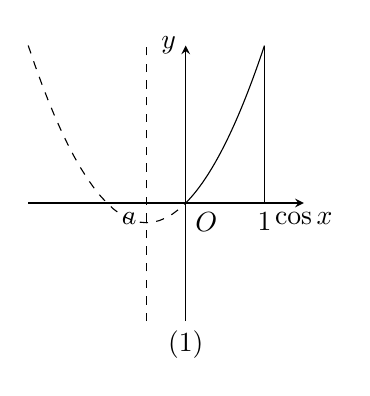
\begin{tikzpicture}[>=stealth]
        \draw [->] (-2,0) -- (1.5,0) node [below] {$\cos x$};
        \draw [->] (0,-1.5) -- (0,2) node [left] {$y$};
        \draw (0,0) node [below right] {$O$};
        \draw [domain = 0:1] plot (\x,{(\x+1/2)^2-1/4});
        \draw [dashed, domain = -2:0] plot (\x,{(\x+1/2)^2-1/4});
        \draw [dashed] (-0.5,-1.5) -- (-0.5,2);
        \draw (1,0) node [below] {$1$} -- (1,2);
        \draw (-0.5,0) node [below left] {$a$};
        \draw (0,-1.5) node [below] {(1)};
    \end{tikzpicture}
    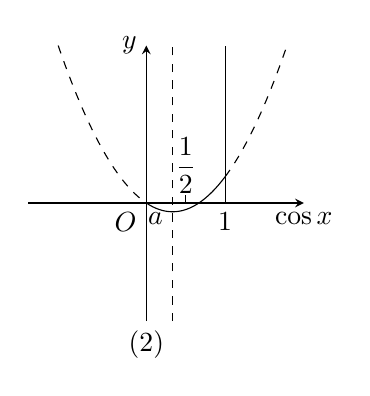
\begin{tikzpicture}[>=stealth]
        \draw [->] (-1.5,0) -- (2,0) node [below] {$\cos x$};
        \draw [->] (0,-1.5) -- (0,2) node [left] {$y$};
        \draw (0,0) node [below left] {$O$};
        \draw [domain = 0:1] plot (\x,{(\x-1/3)^2-1/9});
        \draw [dashed, domain = {1/3-sqrt(2+1/9)}:0] plot (\x,{(\x-1/3)^2-1/9});
        \draw [dashed, domain = 1:{1/3+sqrt(2+1/9)}] plot (\x,{(\x-1/3)^2-1/9});
        \draw [dashed] ({1/3},-1.5) -- ({1/3},2);
        \draw (1,0) node [below] {$1$} -- (1,2);
        \draw ({1/3},0) node [below left] {$a$};
        \draw (0.5,0.1) -- (0.5,0) node [above] {$\dfrac 12$};
        \draw (0,-1.5) node [below] {(2)};
    \end{tikzpicture}
    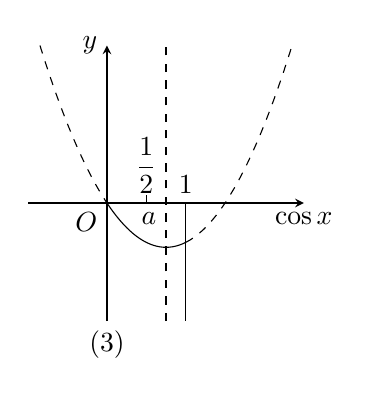
\begin{tikzpicture}[>=stealth]
        \draw [->] (-1,0) -- (2.5,0) node [below] {$\cos x$};
        \draw [->] (0,-1.5) -- (0,2) node [left] {$y$};
        \draw (0,0) node [below left] {$O$};
        \draw [domain = 0:1] plot (\x,{(\x-0.75)^2-9/16});
        \draw [dashed, domain = {0.75-sqrt(2+9/16)}:0] plot (\x,{(\x-0.75)^2-9/16});
        \draw [dashed, domain = 1:{0.75+sqrt(2+9/16)}] plot (\x,{(\x-0.75)^2-9/16});
        \draw [dashed] (0.75,-1.5) -- (0.75,2);
        \draw (1,0) node [above] {$1$} -- (1,-1.5);
        \draw (0.75,0) node [below left] {$a$};
        \draw (0.5,0.1) -- (0.5,0) node [above] {$\dfrac 12$};
        \draw (0,-1.5) node [below] {(3)};
    \end{tikzpicture}
    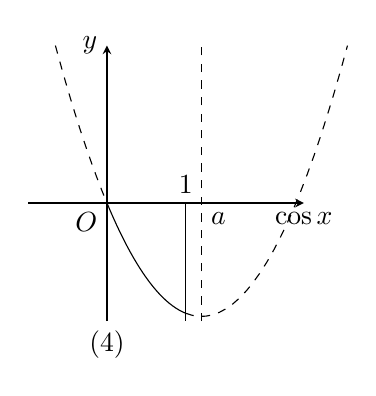
\begin{tikzpicture}[>=stealth]
        \draw [->] (-1,0) -- (2.5,0) node [below] {$\cos x$};
        \draw [->] (0,-1.5) -- (0,2) node [left] {$y$};
        \draw (0,0) node [below left] {$O$};
        \draw [domain = 0:1] plot (\x,{(\x-1.2)^2-1.44});
        \draw [dashed, domain = {1.2-sqrt(2+1.44)}:0] plot (\x,{(\x-1.2)^2-1.44});
        \draw [dashed, domain = 1:{1.2+sqrt(2+1.44)}] plot (\x,{(\x-1.2)^2-1.44});
        \draw [dashed] (1.2,-1.5) -- (1.2,2);
        \draw (1,0) node [above] {$1$} -- (1,-1.5);
        \draw (1.2,0) node [below right] {$a$};
        \draw (0,-1.5) node [below] {(4)};
    \end{tikzpicture}
\end{center}
(1) 如图(1), 此时$a<0$, $m(a)=f(0)=0$, $M(a)=f(1)=1-2a$.\\
(2) 如图(2), 此时$0\le a\le \dfrac 12$, $m(a)=f(a)=-a^2$, $M(a)=f(1)=1-2a$.\\
(3) 如图(3), 此时$\dfrac 12\le a<1$, $m(a)=f(a)=-a^2$, $M(a)=f(a)=0$.\\
(4) 如图(4), 此时$a\ge 1$, $m(a)=f(1)=1-2a$, $M(a)=f(0)=0$.\\
综上所述, 可得$M(a)=\begin{cases}
    1-2a, & a<\dfrac 12,  \\ 0,  & a\ge \dfrac 12,  \end{cases}$ $m(a)=\begin{cases}
    0, & a<0,  \\-a^2, & 0\le a<1,  \\1-2a, & a\ge 1.  \end{cases}$
\item 求函数$y=\dfrac{2\sin x-1}{\sin x+3}$的值域.\\
解答在这里  由已知, 得$\sin x=\dfrac{3y+1}{2-y}$, 而$|\sin x|\le 1$, 故$|\dfrac{3y+1}{2-y}|\le 1$,
即$8y^2+10y-3\le 0$, $(4y-1)(2y+3)\le 0$.  所以函数的值域是$[-\dfrac 32,\dfrac 14]$.
\item 求函数$y=\dfrac{\sec ^2x-\tan x}{\sec ^2x+\tan x}$的值域.\\
解答在这里  因为$\sec ^2x=\tan ^2x+1$, 故原式时变形为$(y-1)\tan ^2x+(y+1)\tan x+(y-1)=0$.\\
(1) 若$y=1$, 则$\tan x=0$.\\
(2) 若$y\ne 1$, 则$\tan x\in \mathbf{R}$, 得$\triangle =(y+1)^2-4(y-1)^2\ge 0$, 于是$\dfrac 13\le y\le 3$且$y\ne 1$.\\
综含(1), (2)知, 函数的值域是$[\dfrac 13,3]$.
\item 解不等式$\sin x\le \dfrac 12$.\\
解答在这里  在单位圆内绘出$\sin x=\dfrac 12$的正弦线(如图), 并结合$y=\sin x$的单调性, 可得$2k\pi -\dfrac{7\pi}6\le x\le 2k\pi +\dfrac{\pi}6$($k\in \mathbf{Z}$).
\begin{center}
    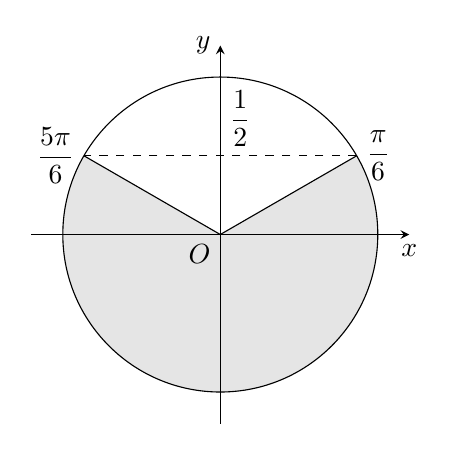
\begin{tikzpicture}[>=stealth,scale = 2]
        \filldraw [gray!20] (0,0) -- (150:1) arc (150:390:1) -- cycle;
        \draw [->] (-1.2,0) -- (1.2,0) node [below] {$x$};
        \draw [->] (0,-1.2) -- (0,1.2) node [left] {$y$};
        \draw (0,0) node [below left] {$O$};
        \draw (0,0) circle (1);
        \draw (30:1) -- (0,0) -- (150:1);
        \draw [dashed] (30:1) -- (150:1);
        \draw (30:1) node [right] {$\dfrac \pi 6$} (150:1) node [left] {$\dfrac {5\pi}6$};
        \draw (0,0.5) node [above right] {$\dfrac 12$};
    \end{tikzpicture}
\end{center}
\item 解不等式$|\cos 2x|\le \dfrac 12$.\\
解答在这里  原不等式为$-\dfrac 12\le \cos 2x\le \dfrac 12$.如图, 可得$k\pi +\dfrac{\pi}3\le 2x\le k\pi +\dfrac{2\pi}3$, 于是$\dfrac{k\pi}2+\dfrac{\pi}6\le x\le \dfrac{k\pi}2+\dfrac{\pi}3$($k\in \mathbf{Z}$).
\begin{center}
    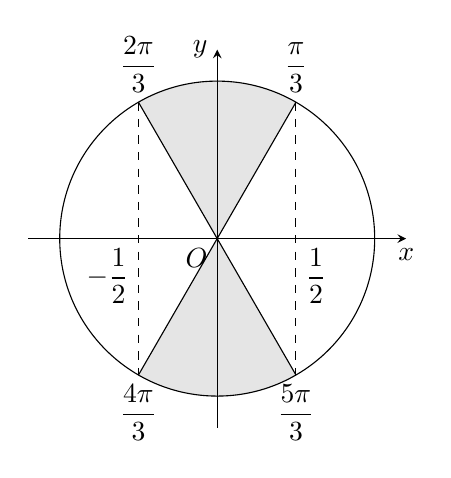
\begin{tikzpicture}[>=stealth,scale = 2]
        \filldraw [gray!20] (0,0) -- (60:1) arc (60:120:1) -- cycle;
        \filldraw [gray!20] (0,0) -- (240:1) arc (240:300:1) -- cycle;
        \draw [->] (-1.2,0) -- (1.2,0) node [below] {$x$};
        \draw [->] (0,-1.2) -- (0,1.2) node [left] {$y$};
        \draw (0,0) node [below left] {$O$};
        \draw (0,0) circle (1);
        \draw (60:1) node [above] {$\dfrac\pi 3$} -- (240:1) node [below] {$\dfrac{4\pi} 3$} (120:1) node [above] {$\dfrac{2\pi} 3$}-- (300:1) node [below] {$\dfrac{5\pi} 3$};
        \draw [dashed] (60:1) -- (300:1) (120:1) -- (240:1);
        \draw (0.5,0) node [below right] {$\dfrac 12$};
        \draw (-0.5,0) node [below left] {$-\dfrac 12$};
    \end{tikzpicture}
\end{center}
\item 解不等式$\tan \dfrac x2\ge \sqrt 3$.\\
解答在这里  如图, 可得$k\pi +\dfrac{\pi}3\le \dfrac x2\le k\pi +\dfrac{\pi}2$,
所以$ 2k\pi +\dfrac{2\pi}3\le x<2k\pi +\pi$($k\in \mathbf{Z}$).
\begin{center}
    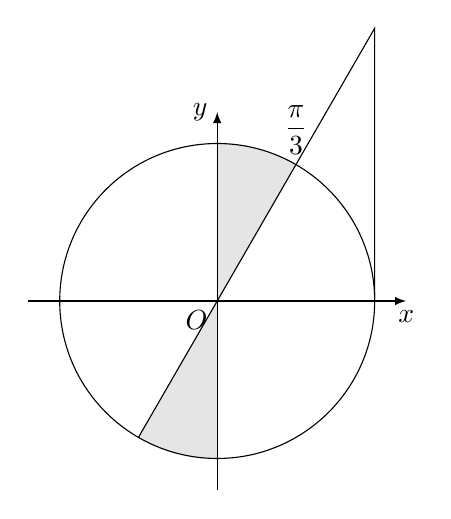
\begin{tikzpicture}[>=latex, scale = 2]
        \filldraw [gray!20] (60:1) arc (60:90:1) -- (0,0) -- cycle;
        \filldraw [gray!20] (240:1) arc (240:270:1) -- (0,0) -- cycle;
        \draw [->] (-1.2,0) -- (1.2,0) node [below] {$x$};
        \draw [->] (0,-1.2) -- (0,1.2) node [left] {$y$};
        \draw (0,0) node [below left] {$O$};
        \draw (0,0) circle (1);
        \draw (240:1) -- (60:2) -- (1,0);
        \draw (60:1) node [above] {$\dfrac \pi 3$};         
    \end{tikzpicture}
\end{center}
\item 在同一个坐标系内, 为了得到$y=3\sin (2x+\dfrac{\pi}4)$的图像, 只需将$y=3\cos 2x$的图像\bracket{20}.
\fourch{向左平移$\dfrac{\pi}4$}{向右平移$\dfrac{\pi}4$}{向左平移$\dfrac{\pi}8$}{向右平移$\dfrac{\pi}8$}
解答在这里  令$f(x)=3\cos 2x$, 则
\begin{align*}f(x-m)&=3\cos 2(x-m)=3\cos (2x-2m)=3\cos (2m-2x)=3\sin [\dfrac{\pi}2-(2m-2x)] \\ &=3\sin (2x+\dfrac{\pi}2-2m).
\end{align*}
按题意应有$3\sin (2x+\dfrac{\pi}2-2m)=3\sin (2x+\dfrac{\pi}4)$.
令$\dfrac{\pi}2-2m=\dfrac{\pi}4$, 得$m=\dfrac{\pi}8$, 故选D.\\
也可以这样解:
因为$f(x)=3\sin (2x+\dfrac{\pi}4)=3\cos [(2x+\dfrac{\pi}4)-\dfrac{\pi}2]=3\cos (2x-\dfrac{\pi}4)=3\cos [2(x-\dfrac{\pi}8)]=f(x-\dfrac{\pi}8)$,
所以选D.
\item 将函数$y=\cos x$图像上每一点的纵坐标保持不变, 横坐标缩小为原来的一半, 再将所得图像沿$x$轴向左平移$\dfrac{\pi}4$个单位长度, 则与所得新图像对应的函数的解析式为\bracket{20}.
\fourch{$y=\cos (2x+\dfrac{\pi}4)$}{$y=\cos (2x-\dfrac{\pi}4)$}{$y=\sin 2x$}{$y=-\sin 2x$}
解答在这里  横坐标缩小为原来的一半, 可理解为伸长到原来的$\dfrac 12$, 故先得到函数$y=\cos \dfrac x{\dfrac 12}=\cos 2x$.再向左平移$\dfrac{\pi}4$后, 得$y=\cos 2(x+\dfrac{\pi}4)$, 即$y=\cos (2x+\dfrac{\pi}2)=-\sin 2x$, 故选D.
\item 函数$y=3\sin x$的图像经过怎样的变换后, 可得到$y=3\sin (\dfrac x2-\dfrac{\pi}4)$的图像?\\
解答在这里 解法一  先``伸缩'', 后``平移''.
第一步: 将函数$y=3\sin x$的图像上的每一点, 纵坐标保持不变, 横坐标伸长到原来的2倍.得到函数$y=3\sin \dfrac x2$的图像.
第二步: 将函数$y=3\sin \dfrac x2$的图像向右平移$\dfrac{\pi}2$个单位长度, 便得到函数$y=3\sin \dfrac 12(x-\dfrac{\pi}2)=3\sin (\dfrac x2-\dfrac{\pi}4)$的图像.\\
解法二  先``平移'', 后``伸缩''.
第一步: 将函数$y=3\sin x$的图像, 向右平移$\dfrac{\pi}4$个单位长度, 得到函数$y=3\sin (x-\dfrac{\pi}4)$的图像.
第二步: 将函数$y=3\sin (x-\dfrac{\pi}4)$的每一点, 纵坐标保持不变, 横坐标伸长到原来的2倍, 得到函数$y=3\sin (\dfrac x2-\dfrac{\pi}4)$的图像.
\item 函数$y=\sin (2x+\dfrac{\pi}4)$图像的一条对称轴是直线\bracket{20}.
\fourch{$x=\dfrac{3\pi}4$}{$x=-\dfrac{3\pi}4$}{$x=\dfrac{3\pi}8$}{$x=-\dfrac{3\pi}8$}
解答在这里 以$x=-\dfrac{3\pi}8$代入, 得$\sin [1(-\dfrac{3\pi}8)+\dfrac{\pi}4]=\sin (-\dfrac{\pi}2)=-1$, 故选D.
\item 若$MP,OM,AT$分别是$60^\circ$角的正弦线、余弦线和正切线, 则\bracket{20}.
\fourch{$MP<OM<AT$}{$OM<MP<AT$}{$AT<OM<MP$}{$OM<AT<MP$}
\item 在同一坐标系内, 曲线$y=\sin x$与$y=\cos x$的交点坐标是\bracket{20}.
\twoch{$(2k\pi +\dfrac{\pi}2,1)$($k\in \mathbf{Z}$)}{$(k\pi +\dfrac{\pi}2,(-1)^k)$($k\in \mathbf{Z}$)}{$(k\pi +\dfrac{\pi}4,\dfrac{(-1)^k}{\sqrt 2})$($k\in \mathbf{Z}$)}{$(k\pi ,0)$($k\in \mathbf{Z}$)}
\item 函数$y=\log _{\frac 12}(\sin 2x)$为减函数的区间是\bracket{20}.
\fourch{$(k\pi ,k\pi +\dfrac{\pi}4]$, $k\in \mathbf{Z}$}{$(k\pi ,k\pi +\dfrac{\pi}2]$, $k\in \mathbf{Z}$}{$(2k\pi ,2k\pi +\dfrac{\pi}4]$, $k\in \mathbf{Z}$}{$(2k\pi ,2k\pi +\dfrac{\pi}2]$, $k\in \mathbf{Z}$}
\item 函数$y=\lg (1-\sin x)-\lg (1+\sin x)$(.)
\twoch{是奇函数, 但非偶函数}{是偶函数, 但非奇函数}{既不是奇函数, 也不是偶函数}{奇偶性无法确定}
\item 若$0<x<\dfrac 12$, 则下列各式不成立的是\bracket{20}.
\fourch{$\sin (1+x)>\sin x$}{$\cos (1+x)<\cos x$}{$(1+x)^x>x^x$}{$\log _x(1+x)>\log _xx$}
\item 若函数$y=\cos (\sin x)$, 则下列结论正确的是\bracket{20}.
\fourch{它的定义域是[-1, 1]}{它是奇函数}{它的值域是$[\cos 1,1]$}{它不是周期函数}
\item 下列四个函数中, 是偶函数且在$[0,\dfrac{\pi}2]$上为增函数, 但不是周期函数的函数是\bracket{20}.
\twoch{$y=|\sin x|$($x\in \mathbf{R}$)}{$y=|\cos x|$($x\in \mathbf{R}$)}{$y=\sin|x|$($x\in \mathbf{R}$)}{$y=|\sin x|+|\cos x|$($x\in \mathbf{R}$)}
\item 下列函数中, 既在$(0,\dfrac{\pi}2)$上是增函数, 又是以$\pi$为最小正周期的偶函数是\bracket{20}.
\fourch{$y=x^2|\cos x|$}{$y=\cos 2x$}{$y=|\sin x|$}{$y=|\sin 2x|$}
\item 要使$\sqrt {(1+2\sin \theta)^2}=-(1+2\sin \theta)$, 则$\theta$的取值范围是\bracket{20}.
\twoch{第三、四象限}{$[2k\pi -\dfrac{5\pi}6,2k\pi -\dfrac{\pi}6]$($k\in \mathbf{Z}$)}{$[2k\pi -\dfrac{\pi}6,2k\pi +\dfrac{7\pi}6]$($k\in \mathbf{Z}$)}{$[2k\pi -\dfrac{7\pi}6,2k\pi -\dfrac{\pi}6]$($k\in \mathbf{Z}$)}
\item 设$\cos ^2x+4\sin x-a=0$($a,x\in \mathbf{R}$), 则$a$的取值范围是\blank{50}.
\item 函数$y=1-2\sin x+3\cos ^2x$的值域是\blank{50}.
\item 函数$y=\sin ^2x+2\cos x(-\dfrac{\pi}3\le x\le \dfrac 23\pi)$的值域是\blank{50}.
\item 函数$y=\dfrac{3\cos x+1}{\cos x+2}$的值域是\blank{50}.
\item 函数$f(x)=\log _{\frac 12}(2\sin x)$的最小值是\blank{50}.
\item 将下列各数由小到大排列: $\sin 46^\circ ,\cos 46^\circ ,\cos 36^\circ$:\blank{50}.
\item 将下列各数由小到大排列: $\sin 2,\cos 2,\tan 2$:\blank{50}.
\item 将下列各数由小到大排列: $\log _x\sin \dfrac x2,\log _x\cos \dfrac x2$($0<x<1$):\blank{50}.
\item 将下列各数由小到大排列: $\cos 1^\circ ,\sin 1^\circ ,\cos 1,\sin 1$:\blank{50}.
\item 在$[0,2\pi]$中, 满足$\sin x\ge \dfrac 12$的$x$的取值范围是\blank{50}.
\item 不等式$\sin x\le \dfrac 12$的解为\blank{50}.
\item 不等式$|\cos 2x|\le \dfrac 12$的解为\blank{50}.
\item 若集合$M=\{\theta|\sin \theta \ge \dfrac 12,0\le \theta \le \pi\}$, $P=\{\theta|\cos \theta \le \dfrac 12,0<\theta \le \pi\}$, 则$M\cap P=$\blank{50}.
\item 若$-\pi \le x\le \pi$, 则不等式$\log _2(1+2\cos x)<1$的解为\blank{50}.
\item 若锐角$\alpha ,\beta$满足$\sin \alpha <\cos \beta$则\bracket{20}.
\fourch{$\alpha >\beta$}{$\alpha <\beta$}{$\alpha +\beta <\dfrac{\pi}2$}{$\alpha +\beta >\dfrac{\pi}2$}
\item 方程$2^x=\cos x$的解有\bracket{20}.
\fourch{$0$个}{$1$个}{$2$个}{无穷多个}
\item 函数$f(x)=(\sin \alpha)^{|\log _{\sin \alpha}x|}$($2k\pi <\alpha <2k\pi +\pi$且$\alpha \ne 2k\pi +\dfrac{\pi}2$, $k\in \mathbf{Z}$)的图像是\bracket{20}.
\fourch{
\begin{center}
    \begin{tikzpicture}[>=stealth]
        \draw [->] (-1,0) -- (2.5,0) node [below] {$x$};
        \draw [->] (0,-1) -- (0,2.5) node [left] {$y$};
        \draw (0,0) node [below left] {$O$};
        \draw [dashed] (1,0) -- (1,1) -- (0,1);
        \draw (1,0) node [below] {$1$} (0,1) node [left] {$1$};
        \filldraw (1,1) circle (0.05);
        \draw [domain = 0.4:2.5] plot (\x,{1/\x});
    \end{tikzpicture}
\end{center}
}{\begin{center}
    \begin{tikzpicture}[>=stealth]
        \draw [->] (-2.5,0) -- (1,0) node [below] {$x$};
        \draw [->] (0,-1) -- (0,2.5) node [left] {$y$};
        \draw (0,0) node [below left] {$O$};
        \draw [dashed] (-1,0) -- (-1,1) -- (0,1);
        \draw (-1,0) node [below] {$-1$} (0,1) node [right] {$1$};
        \draw [domain = 0.4:2.5] plot (-\x,{1/\x});
        \filldraw [fill = white, draw = black] (-1,1) circle (0.05);
    \end{tikzpicture}
\end{center}}{\begin{center}
    \begin{tikzpicture}[>=stealth]
        \draw [->] (-1,0) -- (2.5,0) node [below] {$x$};
        \draw [->] (0,-1) -- (0,2.5) node [left] {$y$};
        \draw (0,0) node [below left] {$O$};
        \draw [dashed] (1,0) -- (1,1) -- (0,1);
        \draw (1,0) node [below] {$1$} (0,1) node [left] {$1$};
        \draw [domain = 0:2.5] plot (\x,\x);
        \filldraw [fill = white, draw = black] (1,1) circle (0.05);
        \filldraw [fill = white, draw = black] (0,0) circle (0.05);    
    \end{tikzpicture}
\end{center}}{\begin{center}
    \begin{tikzpicture}[>=stealth]
        \draw [->] (-1,0) -- (2.5,0) node [below] {$x$};
        \draw [->] (0,-1) -- (0,2.5) node [left] {$y$};
        \draw (0,0) node [below left] {$O$};
        \draw [dashed] (1,0) -- (1,1) -- (0,1);
        \draw (1,0) node [below] {$1$} (0,1) node [left] {$1$};
        \draw (0,0) -- (1,1);
        \draw [domain = 1:2.5] plot (\x,{1/\x});
        \filldraw [fill = white, draw = black] (0,0) circle (0.05);    
    \end{tikzpicture}
\end{center}}
\item 设$x\in (0,\dfrac{\pi}2)$, 则下列各式中正确的是\bracket{20}.
\twoch{$\sin (\sin x)<\cos x<\cos (\cos x)$}{$\sin (\cos x)<\cos x<\cos (\sin x)$}{$\cos (\sin x)<\cos x<\sin (\cos x)$}{$\cos (\cos x)<\cos x<\sin (\sin x)$}
\item 求函数$y=\log _{\sin x}(2\cos x+1)$的定义域.
\item 求函数$y=\sqrt {1-2\cos x}+\lg (2\sin x-\sqrt 2)$的定义域.
\item 求函数$y=\sqrt {\sin x}+\dfrac 1{\sqrt {16-x^2}}$的定义域.
\item 作出函数$y=|\sin x|$的图像.
\item 作出函数$y=|\cos x|+\cos x$的图像.
\item 作出函数$y=(\sin \alpha)^{|\log _{\sin \alpha}x|}$的图像, 其中$\alpha$为锐角.
\item 作出函数$y=\dfrac{|\sin x|}{\sin x}$的图像.
\item 作出函数$y=f(\sin x)$的图像, 其中$f(x)=\begin{cases}
    2, &  x\ge 0,  \\ -1, & x<0. \end{cases}$
\item 若$0<\alpha <\dfrac{\pi}4$, 且$\lg \sin \alpha +\log \cos \alpha +\lg 9=\lg \tan \alpha +\lg \cot \alpha +\dfrac 12\lg 8$, 求$\sin \alpha -\cos \alpha$的值.
\item 设$x$是第二象限角, 且满足$\cos \dfrac x2+\sin \dfrac x2=-\dfrac{\sqrt 5}2$, 求$\sin \dfrac x2-\cos \dfrac x2$的值.
\item 若$0<\theta <\dfrac{\pi}2$, 比较$M=\log _{\sin \theta}\cos \theta$与$N=\log _{\cos \theta}\sin \theta$的大小.
\item 若$\alpha ,\beta$是关于$x$的二次方程$x^2+2(\cos \theta +1)x+\cos ^2\theta =0$的两实根, 且$|\alpha -\beta|\le 2\sqrt 2$, 求$\theta$的范围.
\item 求函数$f(x)=a\sin x-\sin ^2x$的最大值$g(a)$, 并画出$g(a)$的图像.
\item 若函数$f(x)=\cos ^2x-a\sin x+b$的最大值为$0$, 最小值为$-4$, 实数$a>0$, 求$a,b$的值.
\item 函数$y=3\sin (2x+\dfrac{\pi}6)$的图像的一条对称轴是直线\bracket{20}.
\fourch{$x=0$}{$x=\dfrac{\pi}6$}{$x=-\dfrac{\pi}6$}{$x=\dfrac{\pi}3$}
\item 先将函数$y=\sin 2x$的图像向右平移$\dfrac{\pi}3$个单位长度, 再将所得图像作关于$y$轴的对称变换, 则与最后所得图像对应的函数的解析式是\bracket{20}.
\fourch{$y=\sin (-2x+\dfrac{\pi}3)$}{$y=\sin (-2x-\dfrac{\pi}3)$}{$y=\sin (-2x+\dfrac 23\pi)$}{$y=\sin (-2x-\dfrac 23\pi)$}
\item 将函数$y=\sin x$的图像上所有点向左平移$\dfrac{\pi}3$个单位长度, 再把所得图像上各点横坐标伸长到原来的2倍, 则与最后得到的图像对应的函数的解析式为\bracket{20}.
\fourch{$y=\sin (\dfrac x2-\dfrac{\pi}3)$}{$y=\sin (\dfrac x2+\dfrac{\pi}6)$}{$y=\sin (\dfrac x2+\dfrac{\pi}3)$}{$y=\sin (2x+\dfrac{\pi}3)$}
\item 函数$y=A\sin (\omega x+\varphi)$($A>0$, $\omega >0$, $|\varphi|<\dfrac{\pi}2$)的图像如图所示, 则$y$的表达式是\bracket{20}.
\begin{center}
    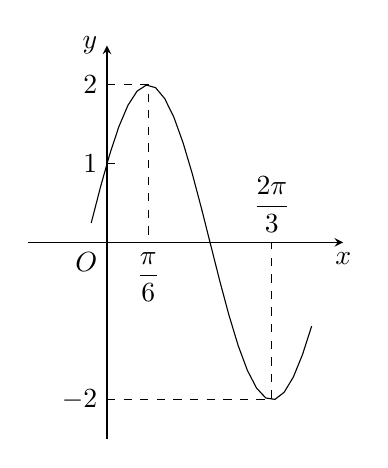
\begin{tikzpicture}[>=stealth]
        \draw [->] (-1,0) -- (3,0) node [below] {$x$};
        \draw [->] (0,-2.5) -- (0,2.5) node [left] {$y$};
        \draw (0,0) node [below left] {$O$};
        \draw [dashed] (0,-2) -- ({2*pi/3},-2) -- ({2*pi/3},0) (0,2) -- ({pi/6},2) -- ({pi/6},0);
        \draw (0.1,1) -- (0,1);
        \draw (0,-2) node [left] {$-2$} (0,1) node [left] {$1$} (0,2) node [left] {$2$} ({pi/6},0) node [below] {$\dfrac \pi 6$} ({2*pi/3},0) node [above] {$\dfrac{2\pi}3$};
        \draw [domain = -0.2:2.6] plot (\x,{2*sin(2*\x/pi*180+30)});
    \end{tikzpicture}
\end{center}
\fourch{$2\sin (\dfrac{10}{11}x+\dfrac{\pi}6)$}{$2\sin (\dfrac{10}{11}x-\dfrac{\pi}6)$}{$2\sin (2x+\dfrac{\pi}6)$}{$2\sin (2x-\dfrac{\pi}6)$}
\item 函数$y=2\sin (\dfrac 12x+\dfrac{\pi}3)$在一个周期内的简图是\bracket{20}.
\fourch{\begin{center}
    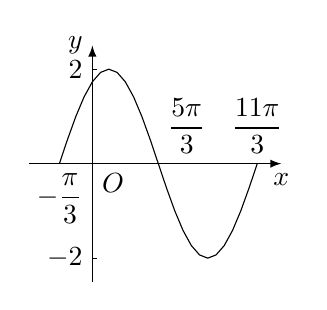
\begin{tikzpicture}[>=latex,yscale = 0.6,xscale = 0.2]
        \draw [->] (-4,0) -- (12,0) node [below] {$x$};
        \draw [->] (0,-2.5) -- (0,2.5) node [left] {$y$};
        \draw (0,0) node [below right] {$O$};
        \draw (0.3,-2) -- (0,-2) node [left] {$-2$};
        \draw (0.3,2) -- (0,2) node [left] {$2$};
        \draw [domain = {-pi*2/3}:{10*pi/3}] plot (\x,{2*sin(\x/2/pi*180+60)});
        \draw ({-2*pi/3},0) node [below] {$-\dfrac \pi 3$};
        \draw ({4*pi/3},0) node [above right] {$\dfrac {5\pi} 3$};
        \draw ({10*pi/3},0) node [above] {$\dfrac {11\pi} 3$};
    \end{tikzpicture}
\end{center}
}{\begin{center}
    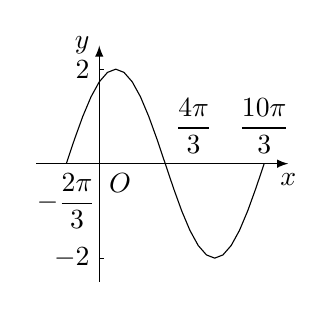
\begin{tikzpicture}[>=latex,yscale = 0.6,xscale = 0.2]
        \draw [->] (-4,0) -- (12,0) node [below] {$x$};
        \draw [->] (0,-2.5) -- (0,2.5) node [left] {$y$};
        \draw (0,0) node [below right] {$O$};
        \draw (0.3,-2) -- (0,-2) node [left] {$-2$};
        \draw (0.3,2) -- (0,2) node [left] {$2$};
        \draw [domain = {-pi*2/3}:{10*pi/3}] plot (\x,{2*sin(\x/2/pi*180+60)});
        \draw ({-2*pi/3},0) node [below] {$-\dfrac {2\pi} 3$};
        \draw ({4*pi/3},0) node [above right] {$\dfrac {4\pi} 3$};
        \draw ({10*pi/3},0) node [above] {$\dfrac {10\pi} 3$};
    \end{tikzpicture}
\end{center}}{\begin{center}
    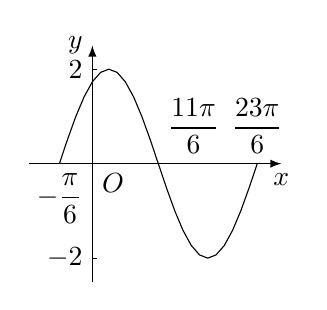
\begin{tikzpicture}[>=latex,yscale = 0.6,xscale = 0.2]
        \draw [->] (-4,0) -- (12,0) node [below] {$x$};
        \draw [->] (0,-2.5) -- (0,2.5) node [left] {$y$};
        \draw (0,0) node [below right] {$O$};
        \draw (0.3,-2) -- (0,-2) node [left] {$-2$};
        \draw (0.3,2) -- (0,2) node [left] {$2$};
        \draw [domain = {-pi*2/3}:{10*pi/3}] plot (\x,{2*sin(\x/2/pi*180+60)});
        \draw ({-2*pi/3},0) node [below] {$-\dfrac \pi 6$};
        \draw ({4*pi/3},0) node [above right] {$\dfrac {11\pi} 6$};
        \draw ({10*pi/3},0) node [above] {$\dfrac {23\pi} 6$};
    \end{tikzpicture}
\end{center}}{\begin{center}
    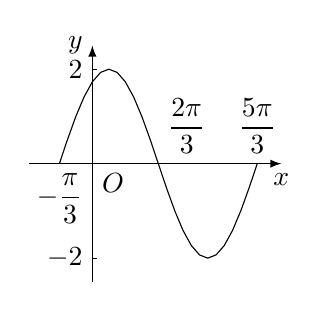
\begin{tikzpicture}[>=latex,yscale = 0.6,xscale = 0.2]
        \draw [->] (-4,0) -- (12,0) node [below] {$x$};
        \draw [->] (0,-2.5) -- (0,2.5) node [left] {$y$};
        \draw (0,0) node [below right] {$O$};
        \draw (0.3,-2) -- (0,-2) node [left] {$-2$};
        \draw (0.3,2) -- (0,2) node [left] {$2$};
        \draw [domain = {-pi*2/3}:{10*pi/3}] plot (\x,{2*sin(\x/2/pi*180+60)});
        \draw ({-2*pi/3},0) node [below] {$-\dfrac \pi 3$};
        \draw ({4*pi/3},0) node [above right] {$\dfrac {2\pi} 3$};
        \draw ({10*pi/3},0) node [above] {$\dfrac {5\pi} 3$};
    \end{tikzpicture}
\end{center}}
\item 要得到函数$y=\sin (\dfrac x2-\dfrac{\pi}6)$的图像, 只需将函数$y=\sin \dfrac x2$的图像\bracket{20}.
\fourch{向右平移$\dfrac{\pi}6$}{向左平移$\dfrac{\pi}6$}{向右平移$\dfrac{\pi}3$}{向左平移$\dfrac{\pi}3$}
\item $f(x)=\log _{\frac{\pi}4}\cos (2x+\dfrac{\pi}4)$为增函数的区间是\blank{50}.
\item 函数$f(x)=2\sin (3-2x)$为增喊数的区间是\blank{50}.
\item 函数$y=\cos (2x-\dfrac{\pi}5)$为减函数的区间是\blank{50}.
\item 函数$y=\sin (2x+\dfrac{\pi}3)$的图像可由$y=\sin 2x$的图像向\blank{50}平移\blank{50}个单位长度得到.
\item 将奇函数$y=f(x)$($x\in \mathbf{R}$)的图像沿$x$轴正向平移$1$个单位长度后, 所得的图像为$C'$, 而图像$C'$与$C$关于原点对称, 那么$C$所对应的函数应为\blank{50}.
\item 先将函数$f(x)=\sin x$的图像向右平移$\dfrac{\pi}5$个单位长度, 再改变各点的横坐标(纵坐标不变), 得到最小正周期为$\dfrac{2\pi}3$的函数$y=\sin (\omega x+\varphi)$($\omega >0$)的图像, 则$\omega =$\blank{50}, $\varphi =$\blank{50}.
\item 若函数$f(x)=2\cos (\dfrac k4x+\dfrac{\pi}3)-5$的最小正周期不大于$2$, 则正整数$k$的最小值为\bracket{20}.
\fourch{$10$}{$11$}{$12$}{$13$}
\item 若函数$f(x)=\sin (2x+\varphi)$($-\pi <\varphi <0$)是偶函数, 则$\varphi =$\blank{50}.
\item 若函数$f(x)=\cos (x+\varphi)$的图像关于坐标原点对称, 则$\varphi =$\blank{50}.
\item 根据周期函数的定义, 求函数$y=2\cos (4x-\dfrac{\pi}3)$的最小正周期.
\item 若奇函数$f(x)$是最小正周期为$3$的周期函数, 且$f(1)=-1$, 则$f(101)=$\blank{50}.
\item 若偶函数$y=f(x)$是最小正周期为$2$的周期函数.且$2\le x\le 3$时, $f(x)=x$, 则当$-2\le x\le 0$时, $f(x)$的表达式为\blank{50}.
\item 已知函数$f(x)=A\sin (\omega x+\varphi)$($A>0$, $\omega >0$)在同一周期内, 当$x=\dfrac{\pi}9$时取得最大值$\dfrac 12$, 当$x=\dfrac{4\pi}9$时取得最小值$-\dfrac 12$, 求此函数的解析式.
\item 已知函数$f(x)=A\sin (\omega x+\varphi)$($A>0$, $\omega >0$)的图像上一个最高点的坐标为$(2,\sqrt 2)$, 由这个最高点到其相邻的最低点间, 图像与$x$轴交于点$(6, 0)$, 求此函数的解析式.
\item 函数$y=\tan 3\pi x$的最小正周期为\bracket{20}.
\fourch{$\dfrac 13$}{$\dfrac 23$}{$\dfrac 6{\pi}$}{$\dfrac 3{\pi}$}
\item 下列函数中, 以$\pi$为最小正周期的偶函数是\bracket{20}.
\fourch{$y=\sin x\cdot \cos x$}{$y=\cot x$}{$y=\cos \dfrac x2$}{$y=\cos ^2x$}
\item 若$a=\sin \dfrac 34$, $b=\cos \dfrac 34$, $c=\cot \dfrac 34$, 则$a,b,c$之间的大小关系是\bracket{20}.
\fourch{$a>b>c$}{$b>c>a$}{$c>a>b$}{$c>b>a$}
\item 若$\tan (2x-\dfrac{\pi}3)\le 1$, 则$x$的取值范围是\bracket{20}.
\twoch{$\dfrac{k\pi}2-\dfrac{\pi}{12}\le x\le \dfrac {k\pi}2+\dfrac 7{24}\pi$($k\in \mathbf{Z}$)}{$k\pi -\dfrac{\pi}{12}\le x<k\pi +\dfrac 7{24}\pi$($k\in \mathbf{Z}$)}{$\dfrac{k\pi} 2-\dfrac{\pi}{12}<x\le \dfrac {k\pi}2+\dfrac 7{24}\pi$($k\in \mathbf{Z}$)}{$k\pi -\dfrac{\pi}{12}<x<k\pi +\dfrac 7{24}\pi$($k\in \mathbf{Z}$)}
\item 下列函数中, 同时满足条件\textcircled{1} 在$(0,\dfrac{\pi}2)$为增函数, \textcircled{2} 为奇函数, \textcircled{3} 以$\pi$为最小正周期的函数是\bracket{20}.
\fourch{$y=\tan x$}{$y=\cot x$}{$y=\tan \dfrac x2$}{$y=|\sin x|$}
\item 函数$y=\cot x(-\dfrac{\pi}4\le x\le \dfrac{\pi}4)$的值域是\bracket{20}.
\fourch{[-1.1]}{$(-\infty ,-1]\cup [1,+\infty)$}{$(-\infty ,-1]$}{$[1,+\infty)$}
\item 已知$x$满足$x$, 则$x$的取值范围为\blank{50}.
\item 已知$x$满足$\tan \dfrac x2\ge \sqrt 3$, 则$x$的取值范围为\blank{50}.
\item 已知$x$满足$\cot 2x\le -\sqrt 3$, 则$x$的取值范围为\blank{50}.
\item 已知$x$满足$|\sin x|\le|\cos x|$, 则$x$的取值范围为\blank{50}.
\item 已知$x$满足$\log _x\tan x>0$, 则$x$的取值范围为\blank{50}.
\item 已知$x$满足$\log _{\sqrt 3}\sin \dfrac x2-\log _{\sqrt 3}\cos \dfrac x2>-1$, 且$-2\pi <x<2\pi$, 则$x$的取值范围为\blank{50}.
\item 将下列各数按从小到大的顺序排列$\tan 1,\tan 2,\tan 3$:\blank{50}.
\item 将下列各数按从小到大的顺序排列$1,\sin 1,\cos 1,\tan 1$:\blank{50}.
\item 在\textcircled{1} $y=|\sin 2x|$, \textcircled{2} $y=|\cos x|$, \textcircled{3} $y=|\tan 2x|$, \textcircled{4} $y=|\tan x|+|\cot x|$这四个函数中, 最小正周期为$\dfrac{\pi}2$的偶函数有\bracket{20}.
\fourch{$0$个}{$1$个}{$2$个}{$3$个}
\item $\sin \dfrac{2\pi}3,\cos 1,\tan 2,\cot 3$的大小关系为\bracket{20}.
\twoch{$\sin \dfrac{2\pi}3>\cos 1>\cot 3>\tan 2$}{$\sin \dfrac{2\pi}3>\cos 1>\tan 2>\cot 3$}{$\cos 1>\sin \dfrac{2\pi}3>\tan 2>\cot 3$}{$\cos 1>\sin \dfrac{2\pi}3>\cot 3>\tan 2$}
\item 若$0<\alpha <2\pi$, 且满足$\sin \alpha <\cos \alpha <\cot \alpha <\tan \alpha$, 则有\bracket{20}.
\fourch{$0<\alpha <\dfrac{\pi}4$}{$\dfrac{\pi}4<\alpha <\dfrac{\pi}2$}{$\pi <\alpha <\dfrac 54\pi$}{$\dfrac{5\pi}4<\alpha <\dfrac{3\pi}2$}
\item 求函数$y=\sqrt {\sqrt 3-\cot \dfrac x2}$的定义域.
\item 求函数$y=\dfrac{\lg (\tan x-1)}{\sqrt {1-2\sin x}}$的定义域.
\item 求函数$y=\lg (\tan x-1)+\sqrt {\sin 2x}$的定义域.
\item 求函数$y=\dfrac{\sec ^2x+\tan x}{\sec ^2x-\tan x}$的值域.
\item 已知$\theta \in [-\dfrac{\pi}3,\dfrac{\pi}4]$, 求函数$y=\sec ^2\theta +2\tan \theta +1$的最大值与最小值.
\item 已知$\dfrac{\pi}3<\theta <\dfrac{\pi}2$, 比较$\sin \theta ,\cot \theta ,\cos \theta$的大小.
\item 已知$0<\alpha <\dfrac{\pi}4$, 比较$\sin \alpha ,\sin (\sin \alpha),\sin (\tan \alpha)$的大小.
\item 已知$0<\theta <\dfrac{\pi}2$, 比较$\cos \theta ,\sin (\cos \theta),\cos (\sin \theta)$的大小.
\item 利用锐角三角函数的定义解决问题``若$\alpha ,\beta \in (0,\dfrac{\pi}2)$, 且$17\cos \alpha +13\cos \beta =17$, $17\sin \alpha =13\sin \beta$, 求$\dfrac{\alpha}2+\beta$''.
\item 利用锐角三角函数的定义解决问题``设$x\in [\dfrac{\pi}4,\dfrac{\pi}2]$, 求证: $\csc x-\cot x\ge \sqrt 2-1$''.
\item 已知$a\cos \alpha +b\sin \alpha =c$, $a\cos \beta +b\sin \beta =c$($0<\alpha ,\beta <\pi$, $\alpha \ne \beta$), 且$\cos \alpha +\cos \beta =\cos \alpha \cdot \cos \beta$, 求证: $c^2-b^2=2ac$.
\item 已知函数$f(x)$满足$af(\sin x)+bf(-\sin x)=c\sin x\cos x(-\dfrac{\pi}2\le x\le \dfrac{\pi}2,a^2-b^2\ne 0)$, 求$f(x)$的解析式.
\item 设$\dfrac{\sin \alpha}{a^2-1}=\dfrac{\cos \alpha}{2a\sin 2\beta}=\dfrac 1{1+2a\cos 2\beta +a^2}$, 求证: $\sin \alpha =\dfrac{a^2-1}{a^2+1}$.
\item 已知$a\sec ^2\alpha -b\cos \alpha =2a$, $b\cos ^2\alpha -a\sec \alpha =2b$, 求$a,b$的关系式.
\item 已知$a\sin ^2\theta +b\cos ^2\theta =m$, $b\sin ^2\varphi +a\cos ^2\varphi =n$, $a\tan \theta =b\tan \varphi$($a,b,m,n$互不相等), 求证: $\dfrac 1m+\dfrac 1n=\dfrac 1a+\dfrac 1b$.
\item 利用单位圆和三角函数线证明:``若$\alpha$为锐角, 则$\sin \alpha +\cos \alpha >1$''.
\item 利用单位圆和三角函数线证明:``若$\alpha$为锐角, 则$\sin \alpha <\alpha <\tan \alpha$''.
\item 利用单位圆和三角函数线证明:``若$\alpha$为锐角, 则$\alpha \cdot \sin \alpha +\cos \alpha >1$''.
\item 利用单位圆和三角函数线证明:``若$0<\beta <\alpha <\dfrac{\pi}2$, 则$\sin \alpha -\sin \beta <\alpha -\beta <\tan \alpha -\tan \beta$''.
\item 若$\alpha$是锐角, 求证: $\cos (\sin \alpha)>\sin (\cos \alpha)$.
\item 已知函数$f(x)$满足$f(x+a)=\dfrac{1-f(x)}{1+f(x)}$($a$为常数, 且$a\ne 0$), 求证: $f(x)$是一个以$2a$为周期的周期函数.
\item 已知$f(x)$为偶函数, 其图像关于直线$x=a$($a\ne 0$)对称, 求证: $f(x)$是一个以$2a$为周期的周期函数.
\item 已知$f(x)$, $g(x)$是定义在$\mathbf{R}$上的两个函数, 且$g(x)$为奇函数.并满足: \textcircled{1} $f(0)=1$; \textcircled{2} 对任何$x,y\in \mathbf{R}$都有$f(x-y)=f(x)f(y)+g(x)g(y)$. 求证:\\
(1) 对任何$x\in \mathbf{R}$都有$f^2(x)+g^2(x)=1$;\\
(2) $f(x)$是偶函数;\\
(3) 若存在非零实数$a$满足$f(a)=1$, 则$f(x)$是周期函数.
\item 利用图像求方程$\sin x=\tan \dfrac x2$在区间$[0,8\pi]$上解的个数.
\item 设$0\le x\le \pi$, $f_1(x)=\sin (\cos x)$, $f_2(x)=\cos (\sin x)$.\\
(1) 求$f_1(x)$, $f_2(x)$的最大值和最小值;\\
(2) 比较$f_1(x)$与$f_2(x)$的大小.
    
\end{enumerate}
\end{document}